\documentclass[12pt]{article}
\usepackage{parskip}
\usepackage[letterpaper, margin=1in]{geometry}
\usepackage{graphicx}
\usepackage{amsmath}
\graphicspath{{./images/}}
\title{ELECENG 2EI5 Lab 3}
\author{Raeed Hassan \\ hassam41 \\  \\ McMaster University}
\date{March 1, 2020}
\begin{document}
\maketitle
\pagebreak

\begin{enumerate}
    \item The photograph of the hardware setup.
    \begin{center}
        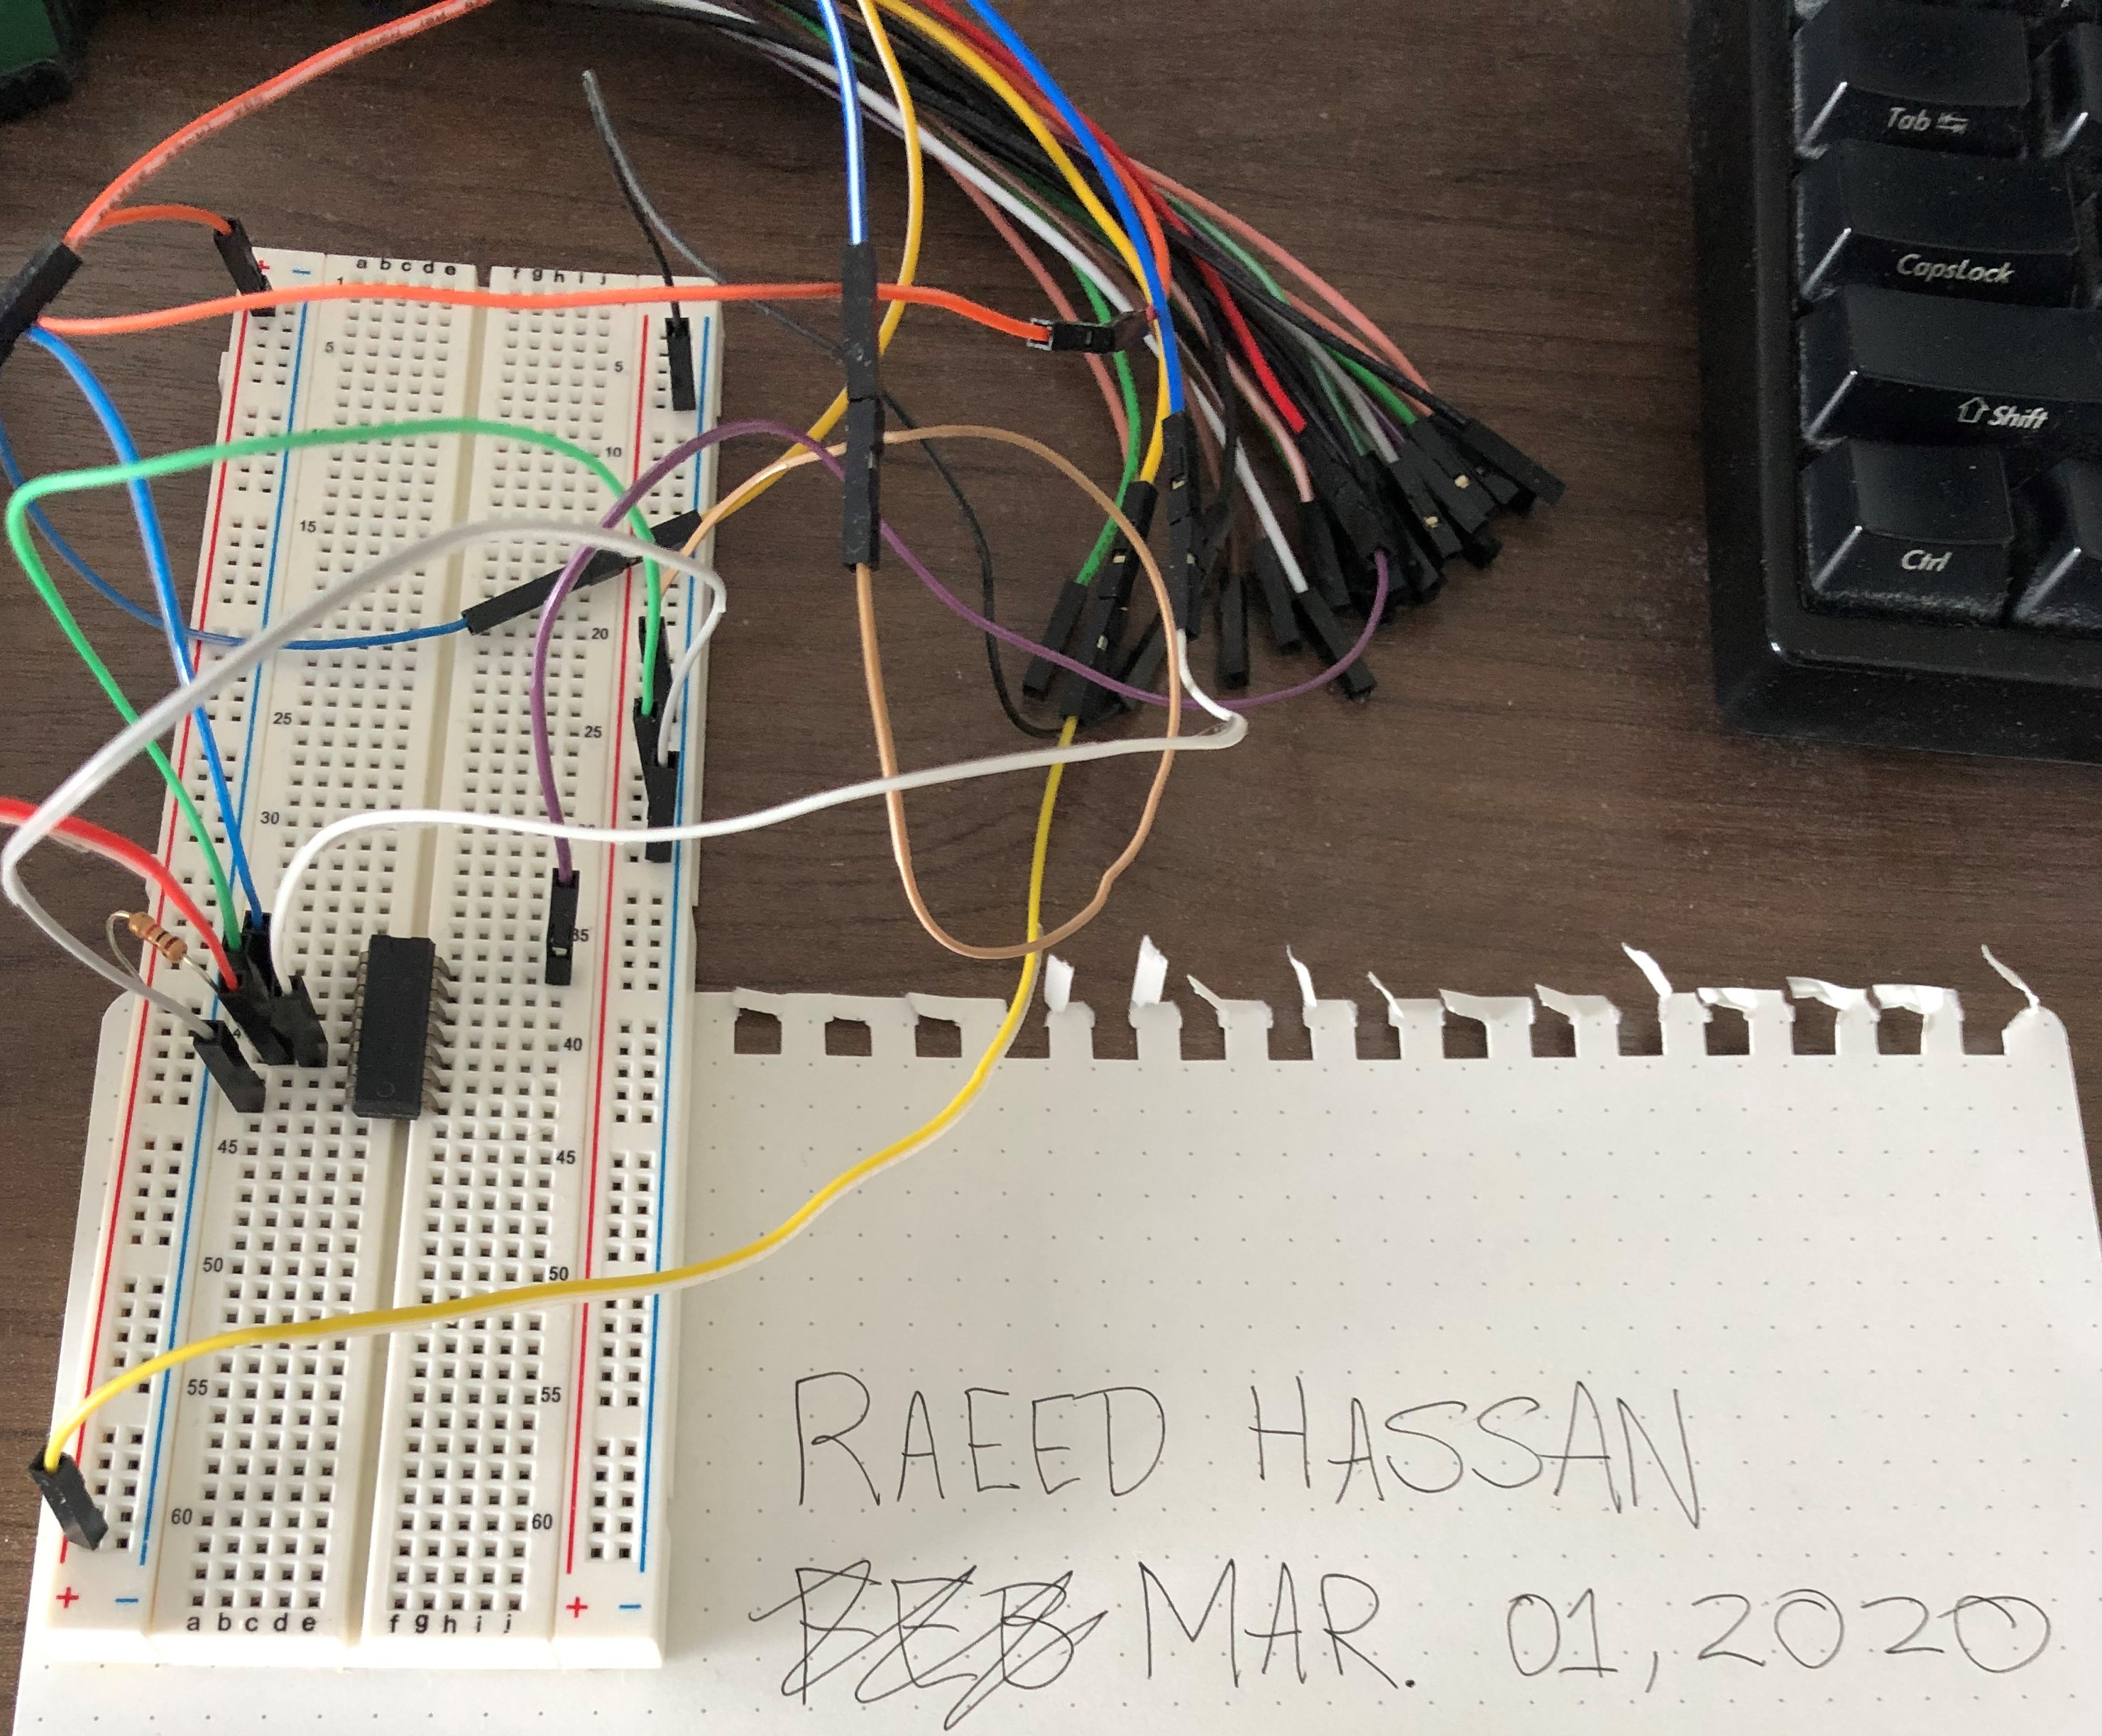
\includegraphics[width=\linewidth]{images/Setup.png}
    \end{center}
    \item Measurement results
    \begin{enumerate}
        \item To measure the current, $i_D$, channel 1 on the oscilloscope measured the voltage across both terminals of a $1k\Omega$ resistor, and a custom math channel, M1, measured the current through the resistor by dividing the voltage in channel 1 by $1000$. For the n-channel MOSFET, the resistor went into the drain and the source was grounded, and for the p-channel MOSFET, the resistor went into the source and the drain was grounded. \pagebreak
        \item
        Figure 1 shows the plot for part a for the n-channel MOSFET.
        \begin{figure}[h!]
            \centering
            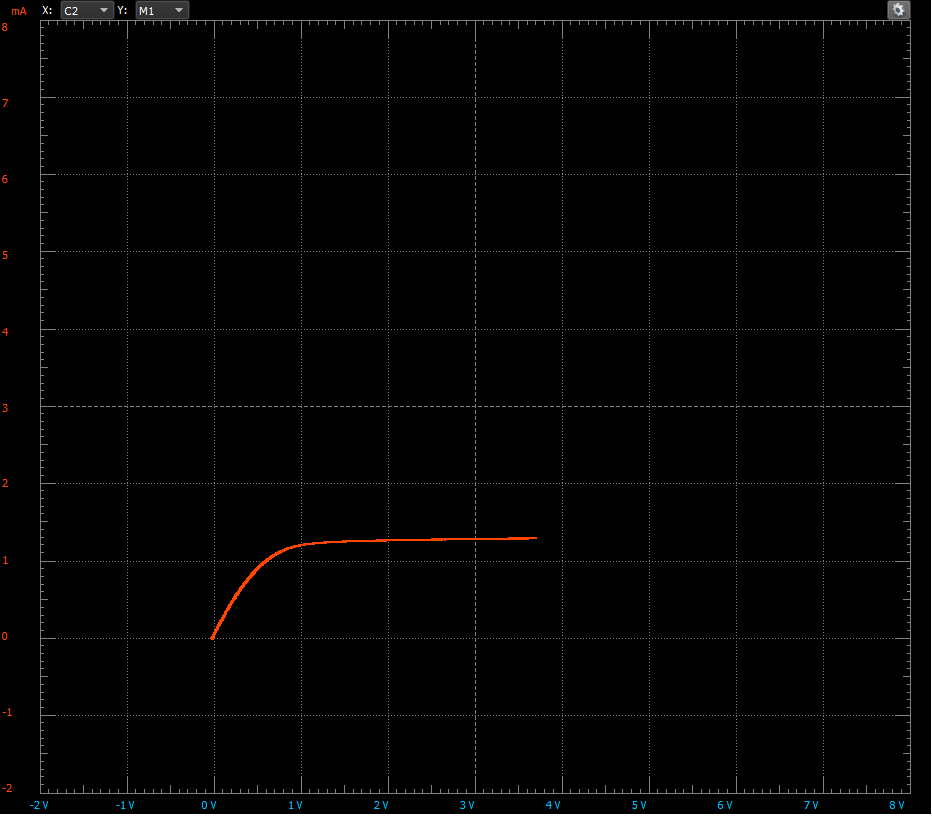
\includegraphics[width=0.5\linewidth]{NAVG3.png}
            \caption{Plot of $i_D$ as function of $v_{DS}$ at $v_{GS} = 4V$ for n-channel MOSFET}
        \end{figure} \\
        Figure 2 shows the plot for part b for the n-channel MOSFET.
        \begin{figure}[h!]
            \centering
            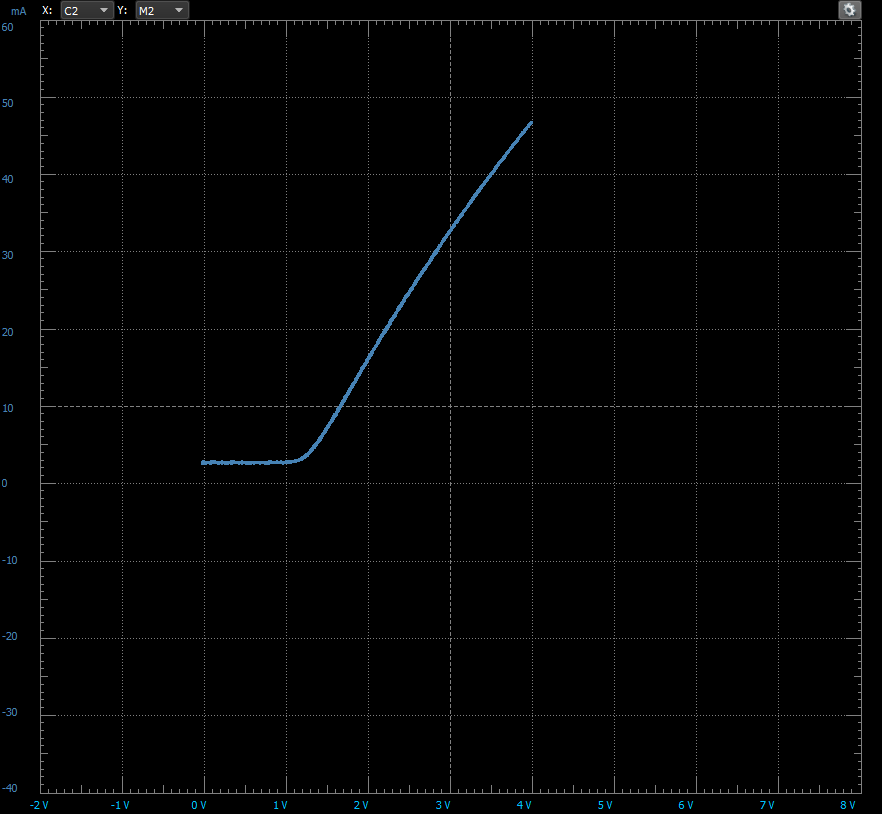
\includegraphics[width=0.5\linewidth]{NBVD5.png}
            \caption{Plot of $i_D$ as function of $v_{GS}$ at $v_{DS} = 5V$ for n-channel MOSFET}                        
        \end{figure} \pagebreak \\
        Figure 3 shows the plot for part c for the n-channel MOSFET.
        \begin{figure}[h!]
            \centering
            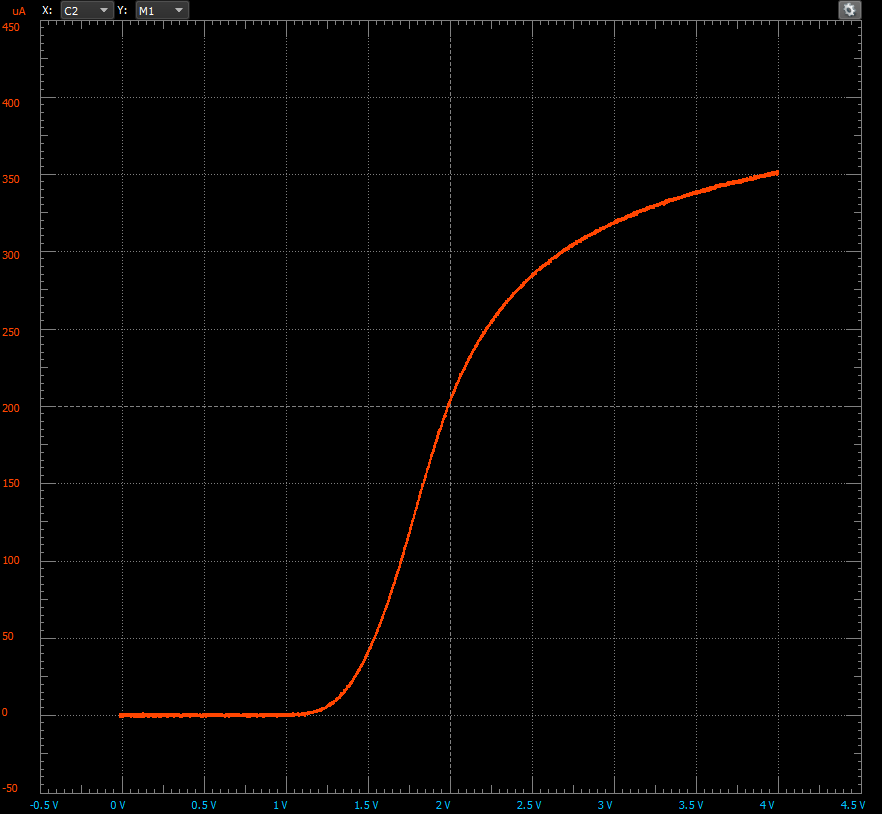
\includegraphics[width=0.5\linewidth]{NCVD50.png}
            \caption{Plot of $i_D$ as function of $v_{GS}$ at $v_{DS} = 0.5V$ for n-channel MOSFET}                        
        \end{figure} \\
        Figure 4 shows the plot for part a for the p-channel MOSFET.
        \begin{figure}[h!]
            \centering
            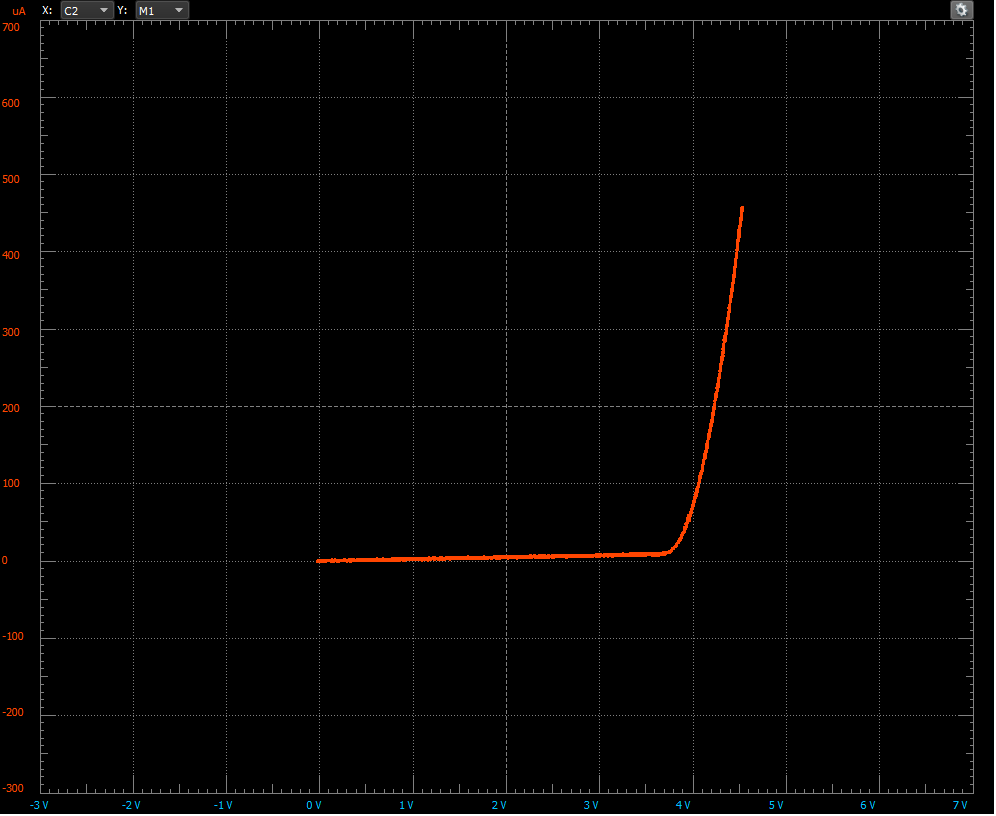
\includegraphics[width=0.5\linewidth]{PAVG3.png}
            \caption{Plot of $i_D$ as function of $v_{SD}$ at $v_{SG} = 4V$ for n-channel MOSFET}                        
        \end{figure} \pagebreak \\
        Figure 5 shows the plot for part b for the p-channel MOSFET.
        \begin{figure}[h!]
            \centering
            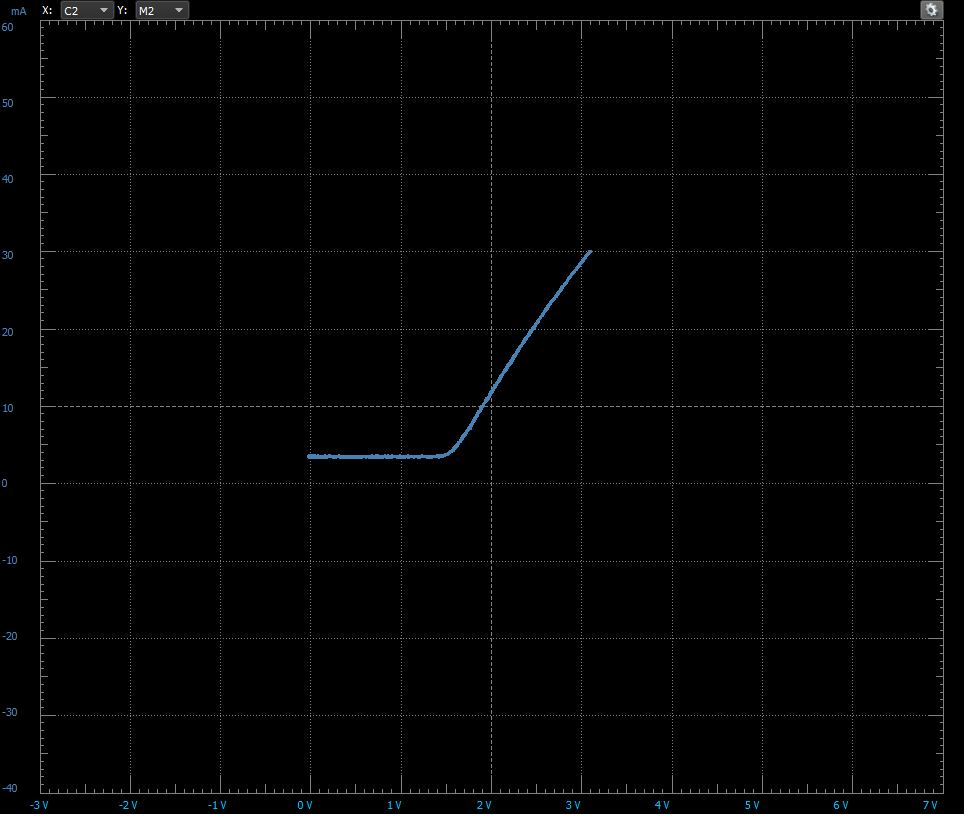
\includegraphics[width=0.5\linewidth]{PBVD5.png}
            \caption{Plot of $i_D$ as function of $v_{SG}$ at $v_{SD} = 5V$ for n-channel MOSFET}                        
        \end{figure} \\
        Figure 6 shows the plot for part c for the p-channel MOSFET.
        \begin{figure}[h!]
            \centering
            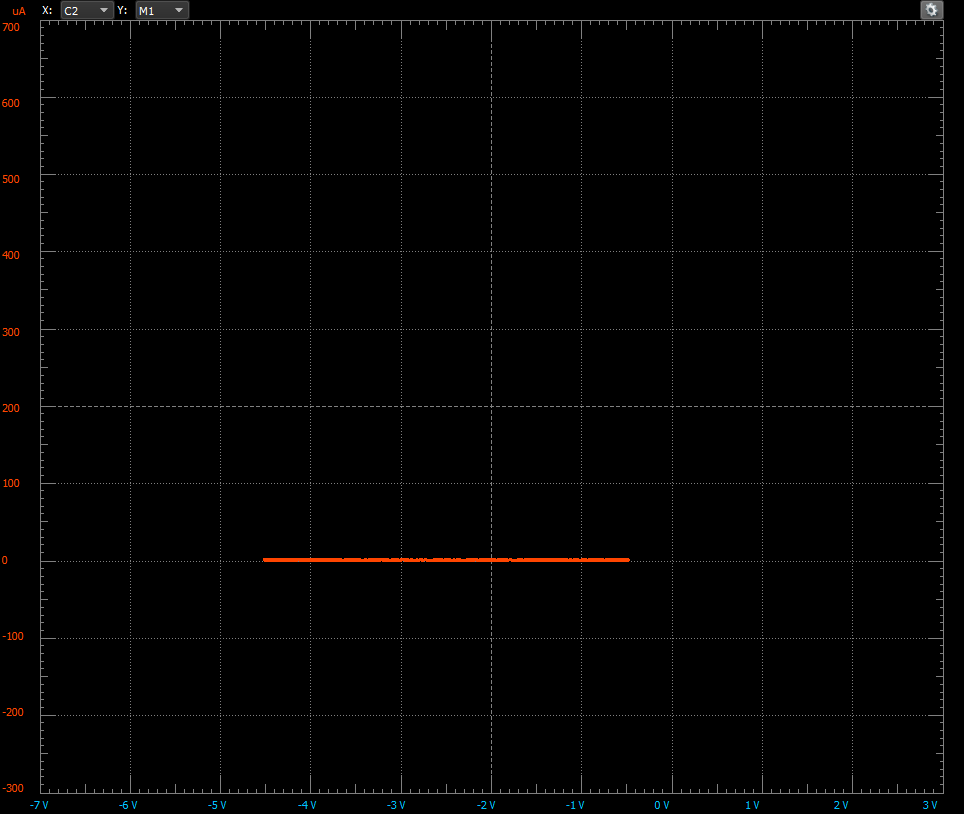
\includegraphics[width=0.5\linewidth]{PCVD50.png}
            \caption{Plot of $i_D$ as function of $v_{SG}$ at $v_{SD} = 0.5V$ for n-channel MOSFET}                        
        \end{figure} \pagebreak
    \end{enumerate}
    The values for $V_T$ can be determined in the plots for part b and c (Figure 2 and 3 for n-channel, Figure 5 and 6 for p-channel), the threshold voltage is the voltage at which graphs have positive current values instead of zero current. The value for $K$ can be determined in the plots for part a (Figure 1 for n-channel, Figure 4 for p-channel), the value of $K$ is twice the slope of the plots in the linear region. 
    \item The shapes of the plots were as expected with little to no discrepancies. Some values did not match in parts b and c, however the reason for this is discussed below in section 4.
    \item For parts b and c, where the value of $v_{DS}$ and $v_{SD}$ had to be set to a certain value, this was not possible using the setup we had. As there had to be a voltage drop across the resistor, the value of $v_D$ or $v_S$ would not be exactly the value that we had for the voltage as the source for the resistor. This meant that some positive voltage values were cutoff with the plots entering negative x-axis values, as can be seen in Figure 6 where the threshold voltage for the p-channel MOSFET is not visible.
\end{enumerate}
\end{document}